\chapter{Convexity and optimization}
\label{chap:optimization}
\thispagestyle{empty}  % Remove opening page number

	Catenaries, Fermat's principle of least time and thermodynamic equilibrium are well known examples of extremum principles applied to the description of nature. On the opposite side, multiple essential modern technologies, such as network routing, logistics and integrated circuit design rely on finding good solutions to optimization problems. No matter whether you are minimizing a Gibbs free energy under constant $T$ and $P$, or searching for the best arrangement of electronic components on a chip to reduce its footprint while satisfying heat dissipation and fabrication constraints, this is what an optimization problem looks like
	%
	\begin{equation}
		p^* = \min \big\{ f_0(x) \mid f_i(x) \leq b_i, \,\forall i \in \{1, \ldots, m\} \big\} .
		\label{eq:optimization-program}
	\end{equation}
	%
	Solving it means finding some $x^* \in \mathbb{R}^n$ such that the value of the \emph{objective function} $f_0(x^*) \leq f_0(x), \,\forall x \in \mathcal{F}$, where
	$$
	\mathcal{F} = \big\{ x \mid f_i(x) \leq b_i , \,\forall i \in \{1, \ldots, m\} \big\}
	$$
	is the \emph{feasible set}. The objective function represents the quantity to be minimized (the free energy; the footprint), while $\mathcal{F}$ imposes the constraints (constant temperature and pressure; rate of heat dissipation and limitations of the fabrication procedure).
	
	Finding global optima for nonlinear programs is difficult, and no robust and efficient general methods to do so are known. That is why one usually consider subsets of eq.~\ref{eq:optimization-program} where some special structure is imposed on the $f_i$. Our goal for this chapter is to learn how to recognize the special structures of linear and semidefinite programs, which requires some groundwork on convexity. Furthermore, polytopes --- a special type of convex sets --- are ubiquitous in the geometry of correlation scenarios, and will make an appearance in later chapters. This will be our starting point.	


	%%%%%%%%%%%%%%%%%%%%%%%%%%%%%%%%%%%%%%
	\section{Convexity}
	\label{sec:convexity}

		This section closely follows the expositions in \cite{rockafellar_convexanalysis_1970,grunbaum_convexpolytopes_2003,ziegler_lecturespolytopes_1995,boyd_convexoptimization_2004}, where most of the alluded proofs can be found. Unless otherwise specified, all sets are subsets of $\mathbb{R}^d$.

		Let $x_1 \neq x_2$ be two elements in $\mathbb{R}^d$. We define
		$$
			\alpha x_1 + (1 - \alpha) x_2, \quad\alpha \in \mathbb{R}
		$$
		as the \emph{line} passing through $x_1$ and $x_2$. A set $A$ containing all lines between pairs of its elements is an \emph{affine set}. The real line and the Cartesian plane are affine sets, but a sphere and a cube are not.

		Finite induction on the definition shows that, for $x_1, \ldots, x_n \in A$ and $\sum_i \alpha_i = 1$, all points $x = \sum_i \alpha_i x_i \in A$.  Such a sum is an \emph{affine combination} of the $x_i$.

		When $A_i$ are affine sets, $A = \bigcap_i A_i$ is also affine. Intersections can only decrease cardinality. Hence, if we take some (not necessarily affine) set $S$ and intersect all possible $A_i \supseteq S$, we will get the smallest affine set containing $S$. This is called an \emph{affine hull}, and denoted $\aff{S}$. Equivalently, it can be shown that
		$$
			\aff{S} = \Big\{ \sum_i \alpha_i x_i \mid \sum_i \alpha_i = 1, \, x_i \in S \Big\} .
		$$
		%
		The affine hull of two points in $\mathbb{R}^n$ is the line through them, and for three noncollinear points we end up with a plane.

		Vector spaces and affine sets are close siblings: any vector space is an affine set, but the converse is not true, for the latter may not contain the $0$ vector. Furthermore, each affine set $A$ is parallel to a unique vector space $V$. Taking any $x_0 \in A$, we can translate $A - x_0 = V$. The \emph{dimension} of an affine space $A$ is the dimension of its parallel vector space $V$. In $\mathbb{R}^n$, dimensions $0, 1, 2$ and $n-1$ corresponds to points, lines, planes and hyperplanes.

		Any hyperplane $H$ can be represented as the set
		$$
			H = \{ u \mid \braket{u}{b} = \beta \} ,
		$$
		where $b \in V$, $\beta \in \mathbb{R}$ are constants, and $\braket{\cdot}{\cdot}$ is an inner product on $V$. Switching from equality to $<, >, \leq$ or $\geq$, we get either open or closed \emph{halfspaces}. Halfspaces contain halflines, so they are not affine sets. Rather, they are convex sets.

		Convex sets are somewhat similar to affine sets. But, instead of lines, a convex set $C$ must contain all \emph{line segments}
		$$
			\alpha x_1 + (1 - \alpha) x_2, \quad\alpha \in [0,1]
		$$
		passing through any $x_1, x_2 \in C$. Any affine set is trivially convex, but a sphere and a cube also are.

		Convex combinations are affine combinations with the extra condition that every $\alpha_i \geq 0$. Likewise, it can be shown that a set $C$ is convex if and only if it contains all convex combinations of its elements. They are also closed under intersections, and the convex hull of a (not necessarily convex) set $S$ is the smallest convex set containing $S$,
		$$
			\conv{S} \equiv \bigcap \big\{ C \supseteq S \mid C \text{ is convex} \big\} .
		$$
		Equivalently, it is also the set of all convex combinations of $S$'s elements,
		%
		\begin{equation}
			\conv{S} = \Big\{ \sum_i \alpha_i x_i \mid \alpha_i \geq 0, \sum_i \alpha_i = 1, \, x_i \in S \Big\} .
		\label{eq:convex-hull}
		\end{equation}
		%
		Convex sets can be further divided into extremal and nonextremal points. An $x \in C$ is an \emph{extreme point} of $C$ when it is not in the relative interior of any segment of $C$; respectively, when $x = \alpha y + (1 - \alpha) z \,\Rightarrow\, x=y=z$ for any $y, z \in C$ and $\alpha \in (0, 1)$.

		\emph{Polyhedra} are intersections of \emph{finitely} many closed halfspaces. Any polyhedron $L \subset \mathbb{R}^d$ can thus be written as
		$$
			L(A, b) = \big\{ x \in \mathbb{R}^d \mid Ax \leq b \big\} ,
		$$
		where $A \in \mathbb{R}^{d \times m}$ and $b \in \mathbb{R}^m$ specify a set of linear inequalities. A single halfspace, which is obviously unbounded, fits the definition. If a polyhedron $L$ is furthermore bounded (i.e., has no rays), it is a convex \emph{polytope}, denoted by $P$. A convex hull of finitely many points is thus a polytope. Polyhedrons and polytopes inherit their dimensions from their affine hull's. From the definition follows that one way to test if an $x \in P$ (or $L$) is to check whether it does not violate any of the inequalities defining the halfspaces. This is closely linked to nonclassicality witnesses, to be further discussed in chap. \ref{chap:pam}.
		%
		\begin{figure*}[t!]
			\newdimen\subfigcapmargin  \subfigcapmargin  =  -3em
			\centering
			\begin{minipage}{.8\textwidth}
				\subfigure[Line]{\label{fig:line}
\includegraphics[width=.16\linewidth]{affine_combination.png}}\hfill
				\subfigure[Segment]{\label{fig:line-segment}
\includegraphics[width=.16\linewidth]{convex_combination.png}}\hfill
				\subfigure[Affine hull]{\label{fig:affine-hull}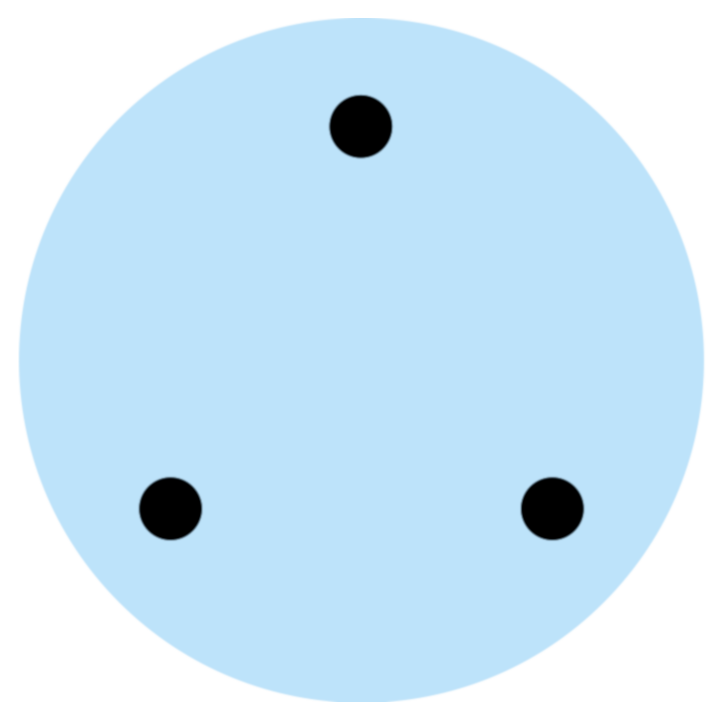
\includegraphics[width=.16\linewidth]{affine_hull.png}}
	
				\subfigure[Convex hull]{\label{fig:convex-hull}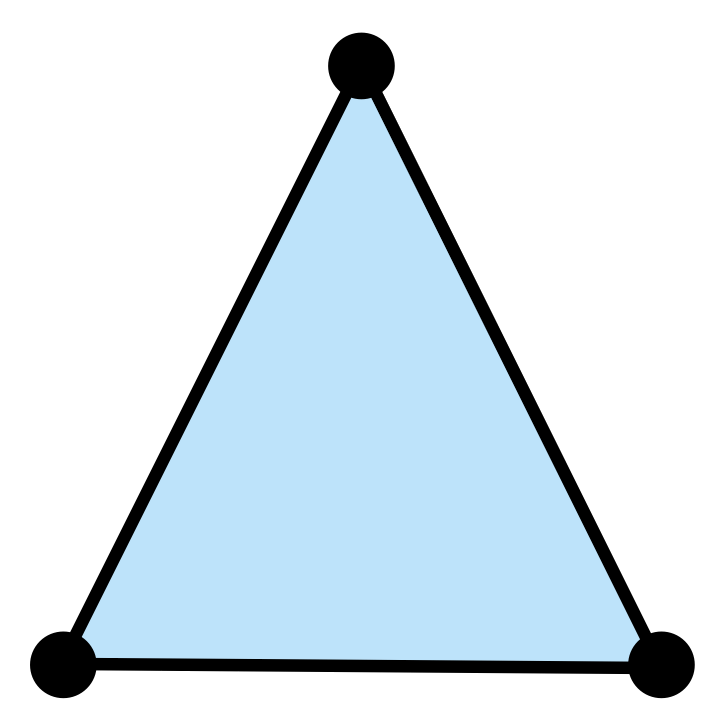
\includegraphics[width=.16\linewidth]{convex_hull.png}}\hfill
				\subfigure[Convex]{\label{fig:convex-not-polytope}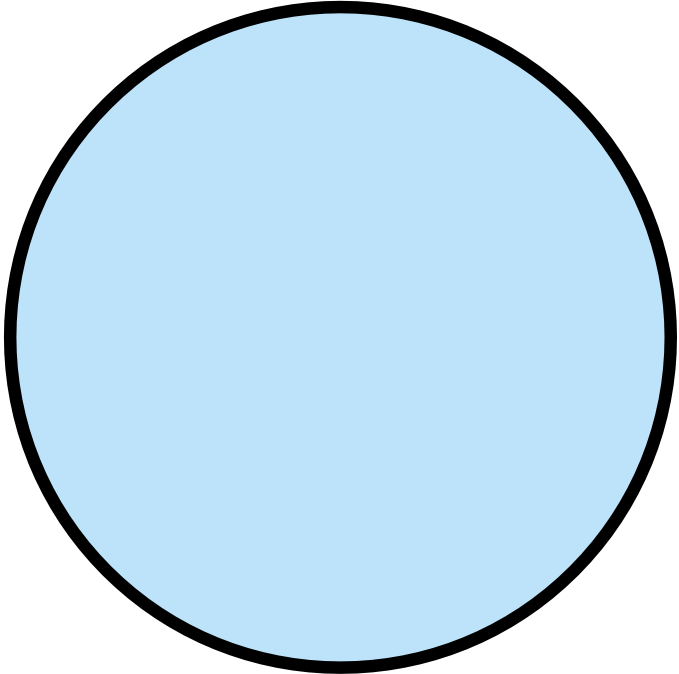
\includegraphics[width=.16\linewidth]{not_polytope.png}}\hfill
				\subfigure[Nonconvex]{\label{fig:nonconvex}
\includegraphics[width=.16\linewidth]{not_convex.png}}
			\end{minipage}
			%
			\caption{Pictorial representation of the definitions introduced in sec. \ref{sec:convexity}. Fig. \ref{fig:line} shows a line, which is an affine combination of two points. In \ref{fig:line-segment}, a line segment between (or a convex combination of) two points is shown. The affine hull of three noncollinear points is the plane (\ref{fig:affine-hull}), while the convex hull of a finite number of points defines a polytope (\ref{fig:convex-hull}). Any polytope is a polyhedron, but the converse is not true. Fig. \ref{fig:convex-not-polytope} shows a convex set with an infinite number of extremal points, therefore not a polytope. Nonconvex sets do not contain every line segment between its elements (\ref{fig:nonconvex}).}
		\end{figure*}


		% \begin{figure}[t!]
		% 	\centering
		% 	\begin{subfigure}{0.3\textwidth}
		% 		
\includegraphics[width=.5\textwidth]{affine_combination.png}}
		% 	\end{subfigure}
		% 	\begin{subfigure}{0.3\textwidth}
		% 		
\includegraphics[height=.13\linewidth]{affine_combination.png}}
		% 	\end{subfigure}
		% 	\begin{subfigure}{0.3\textwidth}
		% 		
\includegraphics[height=.13\linewidth]{affine_combination.png}}
		% 	\end{subfigure}

		% 	\begin{subfigure}{0.3\textwidth}
		% 		
\includegraphics[height=.13\linewidth]{affine_combination.png}}
		% 	\end{subfigure}
		% 	\begin{subfigure}{0.3\textwidth}
		% 		
\includegraphics[height=.13\linewidth]{affine_combination.png}}
		% 	\end{subfigure}
		% 	\begin{subfigure}{0.3\textwidth}
		% 		
\includegraphics[height=.13\linewidth]{affine_combination.png}}
		% 	\end{subfigure}
		% 	%
		% 	\caption{Pictorial representation of the definitions introduced in sec. \ref{sec:convexity}. Fig. \ref{fig:line} shows a line, which is an affine combination of two points. In \ref{fig:line-segment}, a line segment (or a convex hull of two points) is shown. Two affine hull of three noncollinear points is the plane (\ref{fig:affine-hull}), while the convex hull of a finite number of points defines a polytope (\ref{fig:convex-hull}). Any polytope is a polyhedron, but the converse is not true. Fig. \ref{fig:convex-not-polytope} shows a convex set which is not a polytope. Is has an infinite number of extremal points. Nonconvex sets do not contain every line segment between its elements (\ref{nonconvex}).}
		% \end{figure}


		As much as cubes have vertices, edges and faces, polytopes have $k$-faces. Any \emph{face} $F$ of a polytope $P$ is a set
		$$
			F = P \,\cap\, \{ x \in \mathbb{R}^d \mid c^\intercal x = b \} ,
		$$
		where $c \in \mathbb{R}^d$ is a column-vector, $b \in \mathbb{R}$, and any $x \in P$ is such that $c^\intercal x \leq b$. Visually, a face is any intersection of $P$ with a closed halfspace that touches $P$ but is not inside of it. The dimension $k$ of the affine hull of $F$ goes into the name $k$-face. Faces of dimension $0$ and $1$ are vertices and edges, while faces of dimension $\text{dim} (P) - 1$ are especially named \emph{facets}. For a cube ($\mathbb{R}^3$), the facets would match the commonly called faces.

		Our previous definitions of polyhedra and polytopes are sometimes termed $\mathcal{H}$-polyhedra and $\mathcal{H}$-polytopes. An alternative that will later become important is that of $\mathcal{V}$-polytopes, which are defined as the the convex hull of a \emph{finite} set of points. After the convex hull is performed, they become the extremal points of the convex set. The $\mathcal{V}$-description of a unit square is $\mathcal{V} = \{ (0, 0), (1, 0), (0, 1), (1, 1) \}$, and after taking $\conv{\mathcal{V}}$ we get all points that, in the $\mathcal{H}$-description satisfy the linear system $Ax \leq b$ defined by 
		%
		$$
			A =
			\begin{pmatrix}
				-1 & 0 \\
				1 & 0 \\
				0 & -1 \\
				0 & 1
			\end{pmatrix},
			\quad\text{ and }\quad
			b =
			\begin{pmatrix}
				0 \\
				1 \\
				0 \\
				1
			\end{pmatrix} .
		$$
		%

		$\mathcal{H}$ and $\mathcal{V}$ representations can be proven mathematically equivalent (theorem 1.1 in \cite{ziegler_lecturespolytopes_1995}) but, computationally, the choice of description may significantly matter. As will be made explicit in chaps. \ref{chap:pam} and \ref{chap:pam-classical}, classicality in prepare and measure scenarios can be interpreted as the belonging of a behavior in a polytope. Conversely, nonclassicality may be witnessed through the violation of some inequality defining its facets. The $\mathcal{H}$-description of these polytopes is thence preferable for being more ergonomic. Finding these descriptions is important not only for prepare and measure scenarios, but are rather important in several other correlation scenarios. In Bell nonlocality scenarios, for instance, they are the celebrated Bell inequalities. Despite theoretical and practical importance, no general methods to directly build $\mathcal{H}$-descriptions of these polytopes are known. On the other hand, it is conceptually easy to enumerate all extremal points of classicality polytopes (the $\mathcal{V}$-description). Casting one to the other (i.e., performing the vertex or facet enumeration) can be done through specialized, user-friendly softwares such as \texttt{PANDA}, \texttt{lrs} and \texttt{cdd} \cite{PANDA,lrs,cdd} but, unfortunately, this is a computationally expensive problem that can only be done for the very simplest cases of interest. The conceptual significance of $\mathcal{H}$-descriptions will be further explored in chap. \ref{chap:pam}, and an example of description conversion will be discussed in chap. \ref{chap:pam-classical}. Results therein were obtained with \texttt{PANDA}, and descriptions of the algorithms and user guides can be found in the aforementioned references.

		A second important fact involving polyhedra and polytopes is that linear functions can be efficiently optimized inside them through so-called linear programming. In the remainder of this chapter, we go back to the problem posed in the introduction, and briefly discuss two efficiently computable instances of optimization problems, both of which are widely used in quantum information.


	%%%%%%%%%%%%%%%%%%%%%%%%%%%%%%%%%%%%%%%%%%%%
	\section{Optimization}

		Solving an arbitrary instance of eq.~\eqref{eq:optimization-program} is a hard problem, and general methods only exist for special instances of optimization programs. Convex optimization (\texttt{CONV}) --- which happens when all the $f_i$ are convex functions --- is one of the largest classes of programs that can be efficiently solved to global optimality. Even though $\texttt{LIN} \subset \texttt{SDP} \subset \texttt{CONE} \subset \texttt{CONV}$, specialized algorithms for subsets of convex optimization, such as conic (\texttt{CONE}), semidefinite (\texttt{SDP}) and linear (\texttt{LIN}) programming, renders even larger instances of those practical. Whilst we will not discuss them, the main reference for convex programming is the textbook \cite{boyd_convexoptimization_2004}, and a good reference for cone programming, tuned to quantum information, is \cite{uola_conic_2019}.

		Because of their use in the industry, ready-to-use solvers for optimization problems are broadly accessible. I will mention them in due time, but algorithms will not be introduced in depth. For thorough discussions, see, e.g., \cite{papadimitriou1998combinatorial,matousek2007understanding} for linear programming, \cite{vandenberghe_sdp_1996,gartner2012approximation} for SDPs and \cite{boyd_convexoptimization_2004} for convex optimization.


		%%%%%%%%%%%%%%%%%%%%%%%%%%%%%%%%%%%%%%%%%%%%
		\subsection{Linear programming}
		\label{sec:linear-programming}

			Linear programming happens when all the $f_i$ are linear functions. Recalling eq.~\eqref{eq:optimization-program}, you will see that the feasible region $\mathcal{F}$ is thence an intersection of halfspaces --- a polyhedron. Apart from being widely used in the industry to optimize supply chains, workforce allocation and delivery routes, it is also useful to search for probability distributions satisfying a set of constraints. The significance of this problem will become clearer in chap. \ref{chap:pam-classical}.

			Being linear, the objective function $f_0 : \mathbb{R}^n \mapsto \mathbb{R}$ can conveniently be written as $c^\intercal x$, where $c = (c_1, \ldots, c_n)$ is a constant vector in $\mathbb{R}^n$ defining the quantity to be maximized. Minimizing $c^\intercal x$ is the same as maximizing $-c^\intercal x$, so the discussion holds both ways. For an \emph{unconstrained} problem, there is not much more to say: just follow along the direction of the gradient. In this case, though, unless $f_0$ is constant, the program would end up being \emph{unbounded}. Things get more interesting when $x$ is constrained to be in a subset $\mathcal{F} \subset \mathbb{R}^n$. We can do that by saying $0 \leq x_i \leq 1, \,\forall i$, for instance, and then we would be optimizing $c^\intercal x$ over some hypercube. More generally, in linear programming we allow the constraints to be of the form $a_i^\intercal x \leq b_i$, where $a_i \in \mathbb{R}^n$ and $b_i \in \mathbb{R}$. There is no need to consider equality conditions separately, as we can just use two inequalities with inverted directions. So we do not have to write all constraints separately, a shorthand notation is to build an $m \times n$ matrix $A = [a_1 \; \ldots \; a_m]^\intercal$ and a vector $b = [b_1 \; \ldots \; b_m]^\intercal$ of bounds so that
			%
			\begin{subequations}
				\begin{alignat}{2}
					&\text{given}    &\quad & c, A, b \\
					&\underset{x}{\text{max.}}   &	  & c^\intercal x \\
					&\text{s.t.}    &      & Ax \leq b 
				\end{alignat}
				\label{eq:lp}
			\end{subequations}
			%
			is a general form of a linear program (LP). When $\mathcal{F} = \emptyset$, the program is \emph{unfeasible}, meaning there is no vector $x$ that satisfies the constraints. Requiring that $x_i \geq 1$ and $x_i \leq -1$ would certainly put you in that situation. If $\mathcal{F}$ is not empty, then the program may either have a solution or be unbounded. To understand why the latter may be the case, notice that $\mathcal{F}$ is a polyhedron. As such, it may itself be unbounded. Consider, for instance, $x \in \mathbb{R}^2$ with $\mathcal{F} = \{ 0 \leq x_1 \leq 1, x_2 \geq 0 \}$. If $c = [c_1 \; c_2]$, with $c_2 > 0$, the optimal value $p^*$ would go to infinity. On the other hand, $c_2 \leq 0$ would be alright even though $\mathcal{F}$ is unbounded. When $\mathcal{F}$ is a (nonempty) polytope, there is always some solution $p^*$ to the program. A solution is either unique (only a single $x^*$ leads to $p^*$), or there are infinitely many solutions yielding the same $p^*$. To understand why this is so, consider the \emph{fundamental theorem of linear programming}, which states that every feasible, bounded linear program has an optimal solution on a vertex of $\mathcal{F}$. If optimal solutions happen at two different vertices, then any $x$ in the line segment between them results in $p^*$. Otherwise, there would either be a larger feasible value in the segment, or the feasible region would not be convex. 

			Linear programs are efficiently solvable in practice. The simplex method, proposed by George Dantzig in 1947, builds upon the fact that optimal solutions occur in vertices. Starting from any basic feasible solution (a corner of $\mathcal{F}$), it smartly hops to neighboring vertices along edges that increase $f_0$. If you end up at a basic feasible solution connected to no edges that increase the objective value, or if you visit an unbounded edge, you are done. A rigorous presentation and complexity analysis of it can be found in \cite{papadimitriou1998combinatorial}, chap. 2. Interestingly, the simplex method is \emph{not} of polynomial time complexity (i.e., it is not efficient \emph{in theory}). Rather, there are families of linear programs for which it performs poorly. Nevertheless, it is a reliable and efficient method in practice, and is widely used (in several variations) up to this day. There are provably polynomial time algorithms in theory, of which the ellipsoid method --- invented in 1970 for nonlinear programming, then adapted and proved polynomial for linear programming in 1979 ---, was the first. Even so, it is not efficient in practice. The more recent interior-point methods are provably polynomial in theory, and fast in practice. Pedagogical discussions of these methods, together with historical remarks, are nicely presented in chap. 7 of \cite{matousek2007understanding}.

			Due to its wide applicability in the industry, there are many open source and proprietary linear programming solvers available, such as GLPK, Gurobi, and Mosek \cite{glpk,gurobi,mosek}. Most provide user-friendly interfaces to widely used programming languages, such as C, C++, Python and MATLAB. To further aid in using them, there are also modeling languages that can be used to specify programs in a high-level format, and that internally converts and dispatches the problem to specific solvers. YALMIP \cite{yalmip} and CVX \cite{cvx} are widely used inside MATLAB, while PICOS \cite{picos} and CVXPY \cite{cvxpy} are common choices when working in Python.	


		%%%%%%%%%%%%%%%%%%%%%%%%%%%%%%%%%%%%%%%%%%%%
		\subsection{Semidefinite programming}
		\label{sec:sdp}

			Semidefinite programming largely generalizes linear programming, and has found numerous applications in statistics, economics, control theory, pattern recognition and machine learning, to mention a few (see sec. 2 of \cite{vandenberghe_sdp_1996} and chap. 1 of \cite{boyd_convexoptimization_2004} for a survey). It is also widely used as a tool in approximation algorithms to graph theoretical problems \cite{gartner2012approximation}, and polynomial and non-commutative polynomial optimization \cite{npa_prl_2007,npa_njp_2008}; the latter being widely used in quantum information.

			While linear programming is the optimization of a linear function over a polyhedron, semidefinite programming is the optimization of a linear function over a spectrahedron. Before we further explain it, recall that
			$$
				S^m = \{ X \in \mathbb{R}^{m \times m} \mid X = X^\intercal \}
			$$
			is the set of $m \times m$ symmetric matrices, and
			$$
				S_+^m = \{ X \in S^m \mid X \succeq 0 \}
			$$
			the one of positive $m \times m$ semidefinite matrices. All eigenvalues of a symmetric ($X = X^\intercal$) matrix are real, and the positive semidefiniteness condition ($X \succeq 0$) further requires they must be nonnegative.

			Building upon the general linear program~\eqref{eq:lp}, we write a semidefinite program (SDP) as
			%
			\begin{subequations}
				\begin{alignat}{2}
					&\text{given}    &\quad & c, F_0, \ldots, F_n \\
					&\underset{x}{\text{max.}}   &	  & c^\intercal x \\
					&\text{s.t.}    &      & F_0 + \sum_{i=1}^n x_i F_i \succeq 0 .
				\end{alignat}
				\label{eq:sdp}
			\end{subequations}
			%
			Here, $F(x) \equiv F_0 + \sum_{i=1}^n x_i F_i \succeq 0$ is what we call a \emph{linear matrix inequality} (LMI), and it enforces the r.h.s. to be in $S_+^m$. The $n + 1$ matrices $F_0, \ldots, F_n$ are in $S^m$, and we maintain $x \in \mathbb{R}^n$. A semidefinite program is thus the optimization of a linear function $c^\intercal x$ under the constraint that $F(x)$ is positive semidefinite.

			This may seem like a rather arbitrary definition. To debunk this impression, first notice that if $F(x) \succeq 0$ and $F(y) \succeq 0$, then
			$$
				F[ \alpha x + (1 - \alpha) y ] = \alpha F(x) + (1- \alpha) F(y) \succeq 0
			$$
			for all $0 \leq \alpha \leq 1$. Thus, both the objective function and the constraint are convex, and semidefinite programming is a special case of convex optimization. More than that, $S_+^n$ is a convex cone (i.e., it is closed under conic combinations), meaning it is also a special case of conic optimization. Now it does not look that much arbitrary, but rather it seems too specialized. But it is not, for if we let $F_0 = \text{diag}(b)$ and $F_i = \text{diag}(a_i)$, we recover the form of a linear program just like eq.~\eqref{eq:lp}. Putting it all together, $\texttt{LIN} \subset \texttt{SDP} \subset \texttt{CONE} \subset \texttt{CONV}$, as stated in the beginning of this section.

			A general $F(x)$ may have a block-diagonal section of the form $\text{diag}(Ax + b)$, and a more general structure elsewhere. Thus, a linear matrix inequality represents an affine section of $S_+^n$, also called an \emph{spectrahedron}. Unlike polyhedra, they may have curved boundaries. A cylinder, for instance, can be parameterized as an $F(x)$ with $4 \times 4$ matrices \cite{vinzant_spectrahedron_2014}. A last interesting link to linear programming is that $F(x) \succeq 0$ if and only if $z^\intercal F(x) z \geq 0$ for all $z \in \mathbb{R}^m$. An SDP is thus a linear program with infinitely many linear constraints on $x$.

			The usefulness of semidefinite programming in quantum information is hinted by the fact that quantum states and measurement effects are positive semidefinite matrices. As long as the objective function is linear, we can optimize over them, and they have proven to be useful in quantum state discrimination \cite{bae_discrimination_2015}, quantum steering \cite{cavalcanti_2016_steering} and hierarchies for nonlocal correlations \cite{npa_prl_2007,npa_njp_2008}, among other applications. One of them will be shown in chap. \ref{chap:pam-quantum}. A drawback in dealing with density operators or measurement effects is that, while semidefinite programming is, as in here, usually discussed over the real field, quantum objects make use of complex numbers. One can nevertheless embed them in real variables. This can be a cumbersome task to do manually but, luckily, the modeling interfaces mentioned in the last section can do this under the hood before calling the solver.

			Semidefinite programming can also be efficiently solved both in theory and in practice. Interior-point methods are usually robust and efficient, and are implemented in some user-friendly solvers such as SDPA \cite{sdpa} and Mosek \cite{mosek}. Performance comparisons between these and several other SDP solver are available at \cite{performance_sdp_solvers}.


			%%%%%%%%%%%%%%%%%%%%%%%%%%%%%%%%%%%%%
			\subsubsection{Joint measurability robustness}
			\label{sec:incompatibility-robustness}

				The concept of joint measurability was introduced in sec. \ref{sec:measurements}. Following along the same notation, $\mathcal{M} = \{E_b^y \}_{b, y}$ is a set of $Y$ quantum measurements, indexed by $y$, each having $\mathcal{O}(y)$ outcomes. A parent measurement is called $J_\ell$, and only exists if $\sum_\ell J_\ell \delta_{b, \ell_y} = E_b^y$, where $\ell = \ell_1\ell_2\ldots\ell_Y$, and each $\ell_i \in \{ 1, \ldots, \mathcal{O}(i) \}$. From this requirement, it follows that $J_\ell$ can extract all information needed to reproduce $\mathcal{M}$. Whenever such a $J_\ell$ does not exist, $\mathcal{M}$ is incompatible, or not jointly measurable.

				More than determining whether an $\mathcal{M}$ is joint measurable, it is also interesting to ask to what extent a measurement is incompatible. Such \emph{incompatibility robustness} must be defined relative to \emph{something}. This something is what we call a noise model. Formally, a \emph{noise model} $\mathbf{N} : \mathcal{P}(d, \mathbf{n}) \mapsto \mathbb{S}(\mathcal{P}(d, \mathbf{n}))$ maps from the set of $Y = \abs{\mathbf{n}}$ $d$-dimensional POVMs, each with $\mathbf{n} = (n_1, \ldots, n_Y)$ outcomes, to the set $\mathbb{S}(\mathcal{P}(d, \mathbf{n}))$ of subsets of $\mathcal{P}(d, \mathbf{n})$. The simplest possible choice for $\mathbf{N}$ is the white noise model
				%
				$$
					\mathbf{N} = \Bigg\{ \Big\{ \frac{\id}{n_1} \Big\}_{i=1}^{n_1}, \ldots, \Big\{ \frac{\id}{n_Y} \Big\}_{i=1}^{n_Y} \Bigg\} ,
				$$
				%
				but several other common choices, such as depolarization maps or probabilistic noise also fit the definition. In general, it may also depend on $\mathcal{M}$, but we require that it contains at least one set of jointly measurable measurements. Adequateness is a matter of application, and different choices may lead to different results.

				Having the noise model fixed, we define the incompatibility robustness of $\mathcal{M}$, with respect to $\mathbf{N}$, as
				%
				\begin{equation}
				    \chi^*_\mathcal{M} = \sup_{\substack{\chi \,\in\, [0, 1]\\ \{ N_{b \mid y}\} \,\in\, \textbf{N}( \mathcal{M} )}} \Big\{ \chi \mid \chi \{ E_{b \mid y} \} + (1 - \chi) \{ N_{b \mid y} \} \in \textbf{JM} \Big\} .
				    \label{eq:incompatibility-robustness}
				\end{equation}
				%
				$\textbf{JM}$ denotes the set of all jointly measurable measurements, and $\chi^*_\mathcal{M} = 1$ readily implies $\mathcal{M}$ is jointly measurable. Any lower value means it is not, for to become it must be mixed with noise. More than that, if $\chi^*_\mathcal{M} < \chi^*_{\mathcal{M}^\prime}$ then $\mathcal{M}$ is \emph{more} incompatible than $\mathcal{M}^\prime$.

				Incompatibility robustness was investigated and applied in several works involving quantum measurements and more general quantum devices, such as \cite{heinosaari_noiserobustness_2015,designolle_robustness_2019,uola_onetoonesteering_2015}. Our presentation follows the very thorough investigation in \cite{designolle_robustness_2019}, where analytical and numerical results for several noise models are presented, and further references can be found. The fact that eq.~\eqref{eq:incompatibility-robustness} can be solved through semidefinite programming is also known. To see why this is so, first notice that, if we take a closed noise set, the supremum in \eqref{eq:incompatibility-robustness} becomes a maximum. Furthermore, $f_0 = \chi$, so we are indeed optimizing a linear function. The measurement effects, $\{ E_{b \mid y} \}$ and noise effects $\{ N_{b \mid y} \}$ are given, and $J_\ell$, an optimization variable, is a collection of PSD operators (i.e., the parent measurement's effects). They must be constrained to sum to the identity, and the parent's marginals must recover $\mathcal{M}$. These are semidefinite constraints, as more clearly seen by writing the program
				%
				\begin{subequations}
					\begin{alignat}{2}
						&\text{given}    &\quad &\{ E_{b \mid y} \}, \{ N_{b \mid y} \} \\
						&\underset{\chi, J_\ell}{\text{max.}}   &	  & \chi \\
						&\text{s.t.}    &      &  \sum_\ell J_\ell \delta_{b, \ell_y} = \chi E_{b \mid y}  + (1 - \chi) N_{b \mid y}, \quad\forall b, y \\
						&				&		& J_\ell \succeq 0 \\
						&				&		& \chi \leq 1 .
					\end{alignat}
					\label{eq:incompatibility-robustness-sdp}
				\end{subequations}
				%
				Notice that the constraints $\eta \geq 0$ and $\sum_\ell J_\ell = \id$ are not missing, but rather are automatically enforced by the first constraint and the fact that the noise set must have at least one jointly measurable element, such that $0$ will always be a lower bound. We will come back to this program in sec. \ref{sec:incompatibility-vs-classicality}, where it will be crucial to our proof that measurement incompatibility is not sufficient for nonclassicality in prepare and measure scenarios. Before getting to that, we must first learn what prepare and measure scenarios actually are.